\begin{figure}[t]
	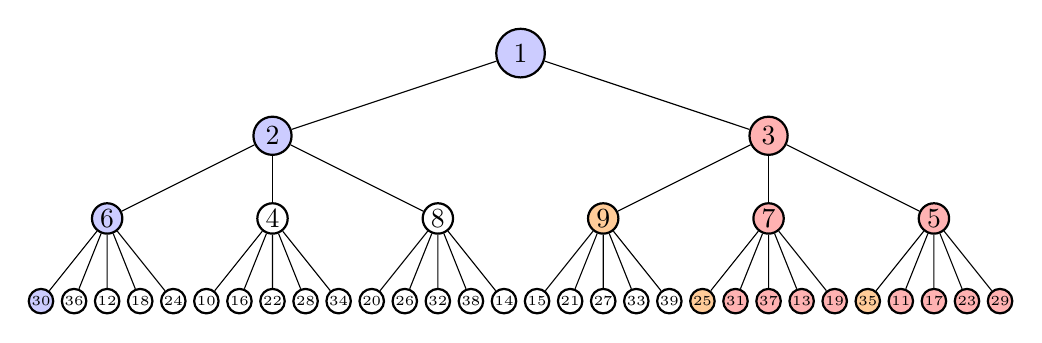
\begin{tikzpicture}[level distance=1.5cm, scale=0.7, level 0/.style={inner sep=2.5pt}, level 1/.style={sibling distance=9cm, inner sep=2pt}, level 2/.style={sibling distance=3.0cm, inner sep=1pt}, level 3/.style={sibling distance=0.6cm, inner sep=0.5pt}]
	\tikzstyle{every node}=[circle,draw,thick]

	\node (Root) [fill=blue!20] {1}
		child { node [fill=blue!20] {2} 
			child { node [fill=blue!20] {6} 
				child { node [fill=blue!20] {\tiny 30} }
				child { node {\tiny 36} }
				child { node {\tiny 12} }
				child { node {\tiny 18} }
				child { node {\tiny 24} }
			}
			child { node {4}
				child { node {\tiny 10} }
				child { node {\tiny 16} }
				child { node {\tiny 22} }
				child { node {\tiny 28} }
				child { node {\tiny 34} }
			}
			child { node {8}
				child { node {\tiny 20} }
				child { node {\tiny 26} }
				child { node {\tiny 32} }
				child { node {\tiny 38} }
				child { node {\tiny 14} }
			}
		}
		child { node [fill=red!30] {3}
			child { node [fill=orange!40] {9}
				child { node {\tiny 15} }
				child { node {\tiny 21} }
				child { node {\tiny 27} }
				child { node {\tiny 33} }
				child { node {\tiny 39} }
			}
			child { node [fill=red!30] {7}
				child { node [fill=orange!40] {\tiny 25} }
				child { node [fill=red!30] {\tiny 31} }
				child { node [fill=red!30] {\tiny 37} }
				child { node [fill=red!30] {\tiny 13} }
				child { node [fill=red!30] {\tiny 19} }
			}
			child { node [fill=red!30] {5}
				child { node [fill=orange!40] {\tiny 35} }
				child { node [fill=red!30] {\tiny 11} }
				child { node [fill=red!30] {\tiny 17} }
				child { node [fill=red!30] {\tiny 23} }
				child { node [fill=red!30] {\tiny 29} }
			}
		};
	\end{tikzpicture}
	\caption{The Sequential Prime Modulus Tree\label{fig:spmt1}}
\end{figure}
